\section{Calculated Inputs}
\label{sec:usingStatisticalInput}
As described in the Section~\ref{sec:annSection} and in Figure~\ref{fig:overfitting} the Neural Network strives for a generalized function without over-fitting so that it also applies for data outside of the trained set. In order to achieve such a function it is necessary to include enough input parameters to get a close enough fit. Every input parameter should narrow down the possible number of output values and add more characteristics of the output to predict, e.g. wind power and electricity prices. The seasonal changes caused by consumer behaviour (holiday, night and day, summer, ect.) and shift in weather conditions contribute heavily to difference in demand and the wind power and price development of the underlying market \cite{yamin2004adaptive,forecastingSpotPricesAccountingForWindPower}. The ability to identify and adapt to these trends are very important and the Artificial Neural Networks attempts to capture all of this in its generalization function. The electricity prices and wind power productions are very volatile and the trends shift constantly and the more characteristics of the trend shifts we can give the ANN to generalize upon the better it can potentially approach its target. It is apparent from Figures~\ref{fig:priceHourDevelopment400HoursStatistics} and~\ref{fig:windHourDevelopment400HoursStatistics} that price follows certain trends and what comes next is highly influenced by the immediate previous hours (also discussed in Section~\ref{sec:historicalData}). 

\begin{figure}[H]
\centering
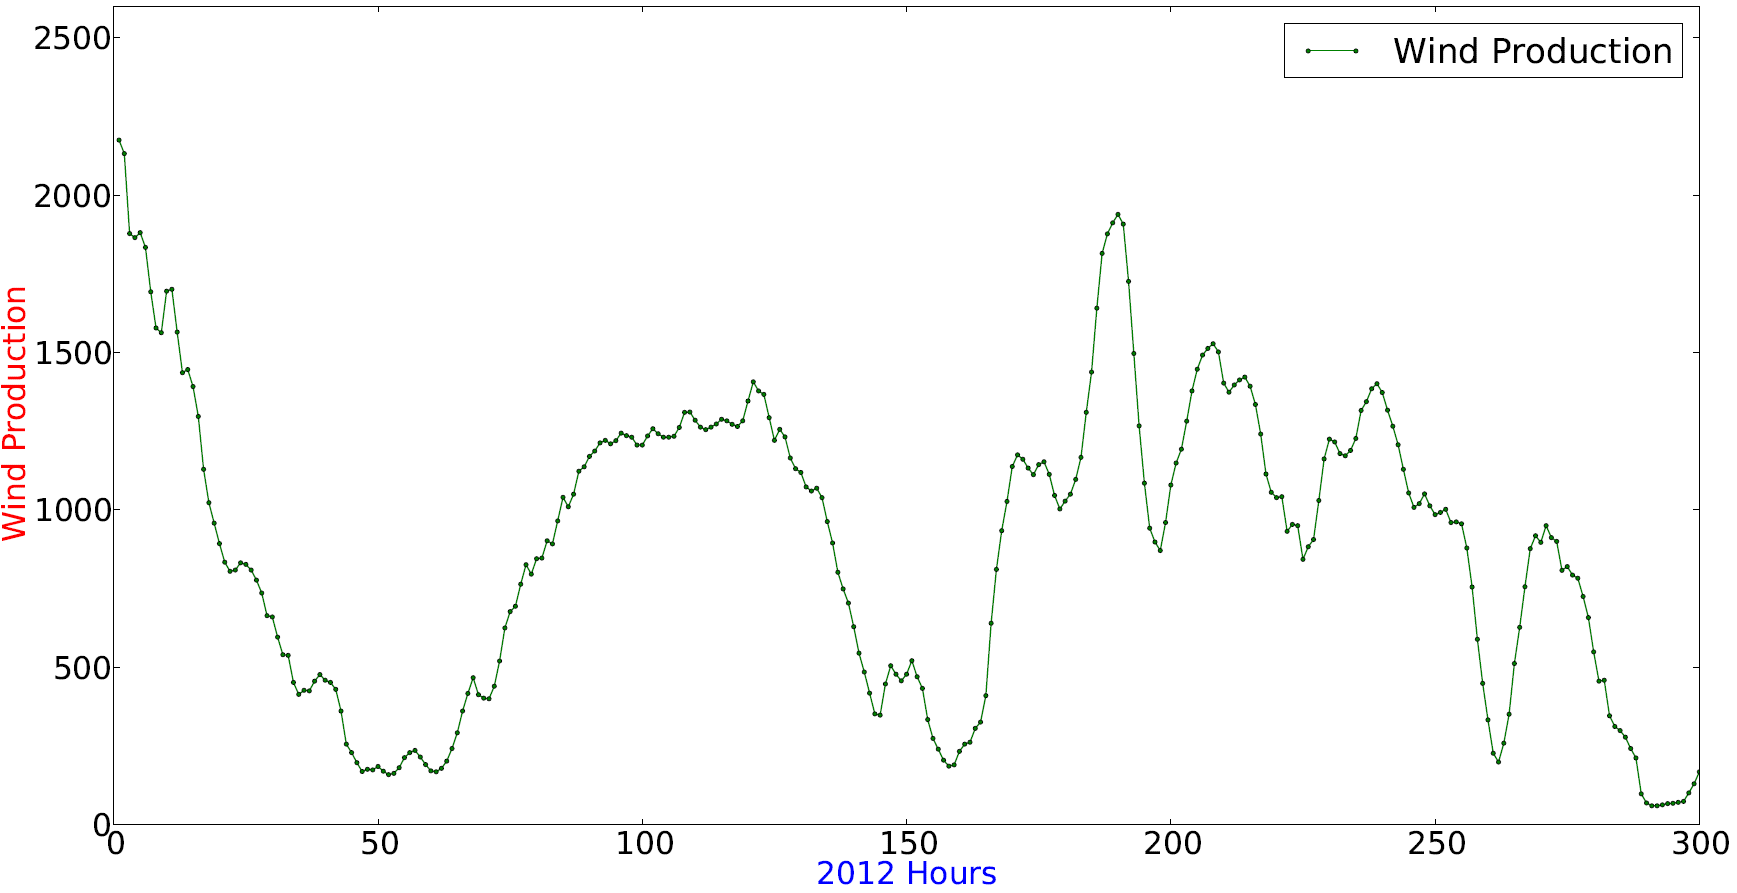
\includegraphics[width=0.99\linewidth,natwidth=898,natheight=587]{billeder/productionTendency400Hours.png}
\caption{Wind production development for 400 hours in 2011}
\label{fig:windHourDevelopment400HoursStatistics}
\end{figure}

\begin{figure}[H]
\centering
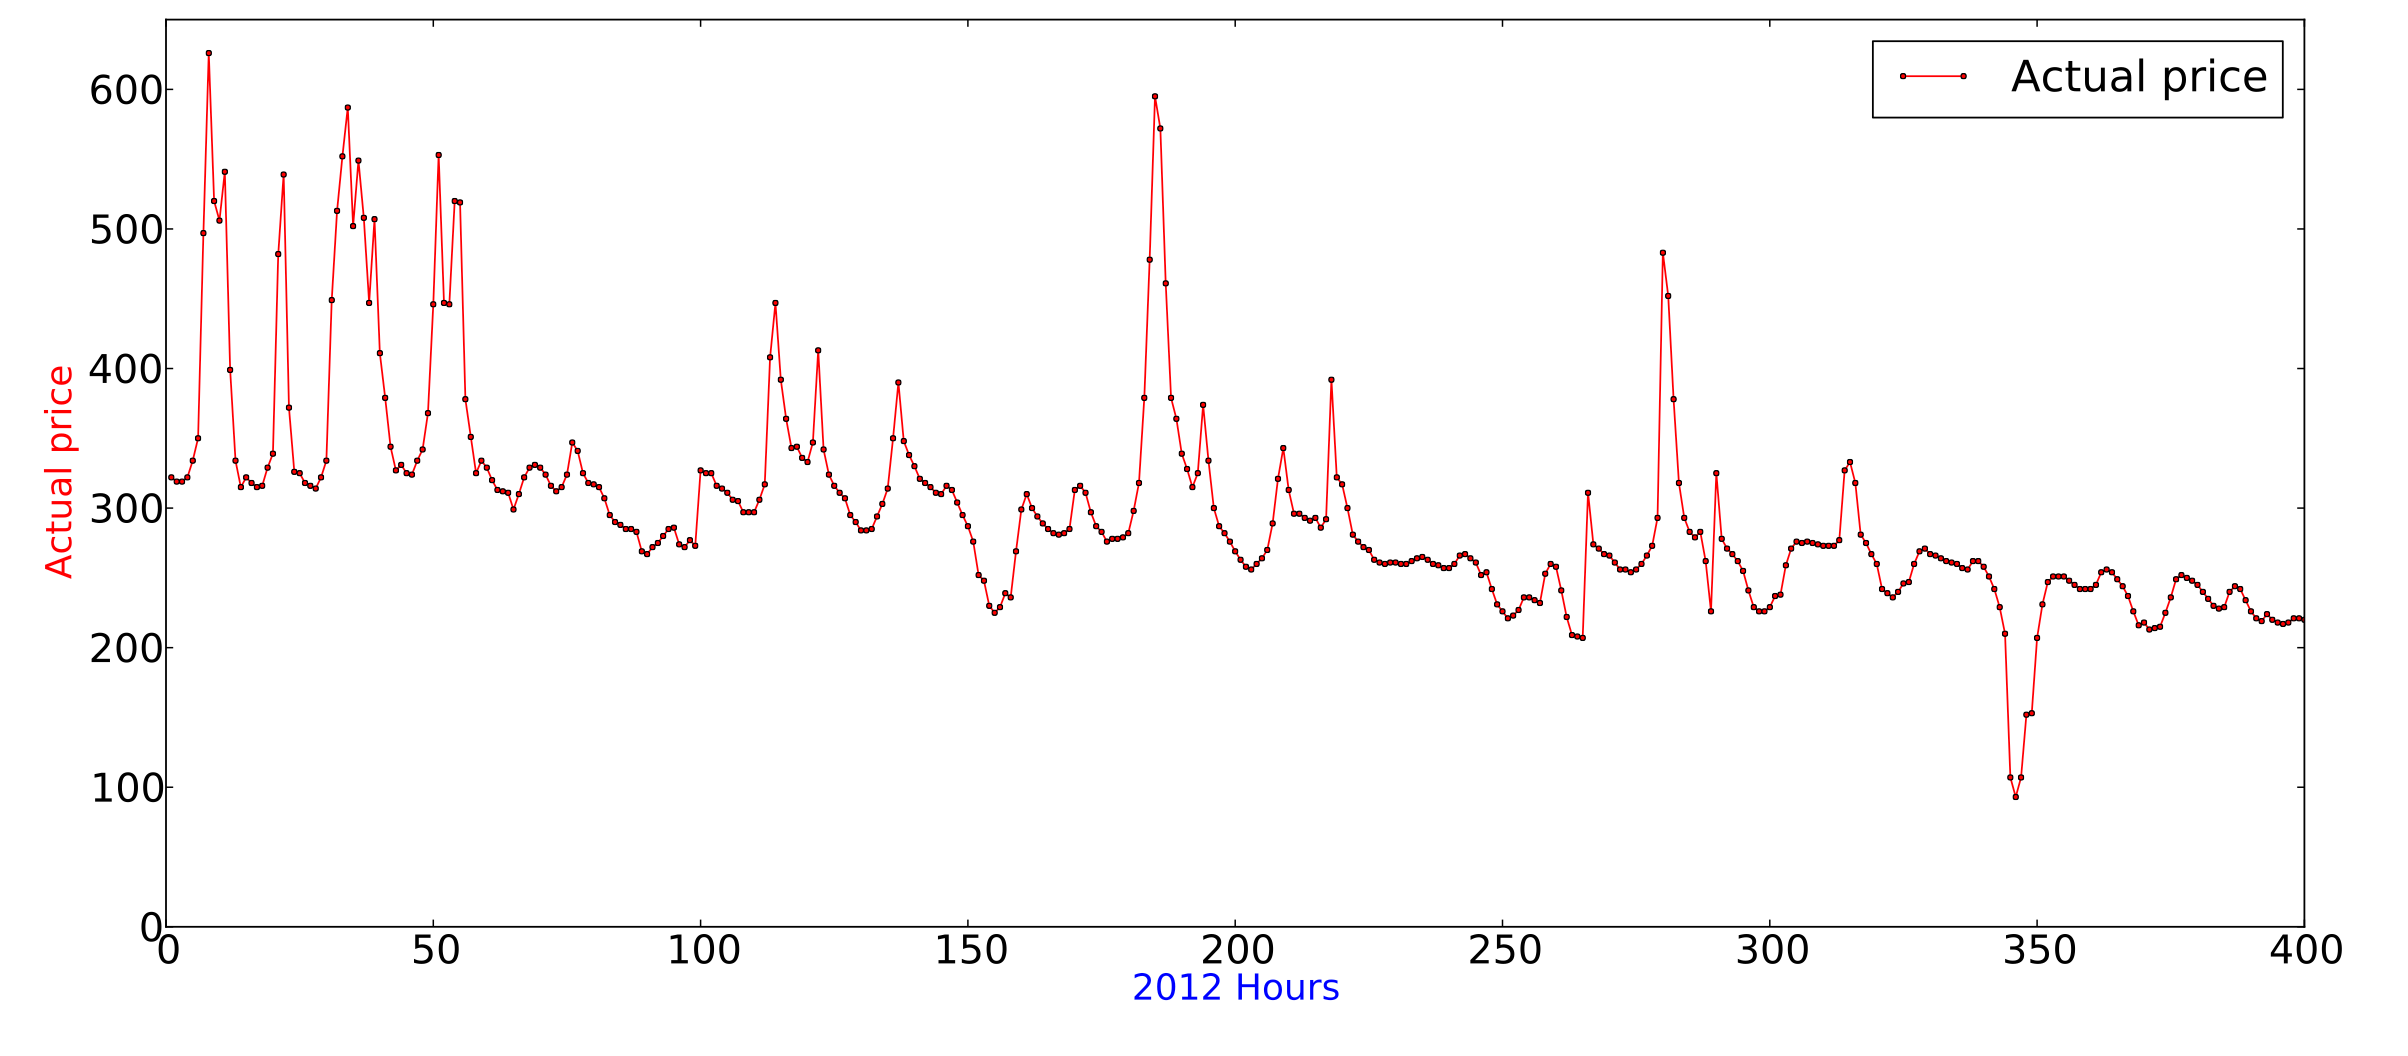
\includegraphics[width=0.99\linewidth,natwidth=898,natheight=587]{billeder/priceGraph400.png}
\caption{Price development for 400 hours in 2012}
\label{fig:priceHourDevelopment400HoursStatistics}
\end{figure}

The prerequisite for adding trend as input is the existence of a general recognizable pattern between the immediate past hours and the hours to predict so that the network through the dataset can identify its influence. The section~\ref{sec:windPowerWindSpeed} shows how the same wind speed can respond to an interval of wind power production, e.g. wind speed 15 equals to productions between 700-1800. The generalization function would give a result to the benefit of the majority but by including trend or volatility as input the idea is to point the generalization in the right direction within this interval, e.g. if the wind speed 15 has equaled 1500-1800 in wind power through the entire training set but the hour we are predicting in the testing set has a last known wind power of 1300 and the trend is descending then the prediction should probably not be between 1500-1800 according to similar descending. The approach of calculating the behavior or trend based on previous hours is applicable for 24-step-ahead forecasting since it can smooth out the transition between the training set and the testing set by grounding the prediction hours in previous ideal values. The point is to take the existing generalization and making it approach better by adding additional inputs --- Figure~\ref{fig:WP} attempts to visualize this. 

\begin{figure}[H]
\centering
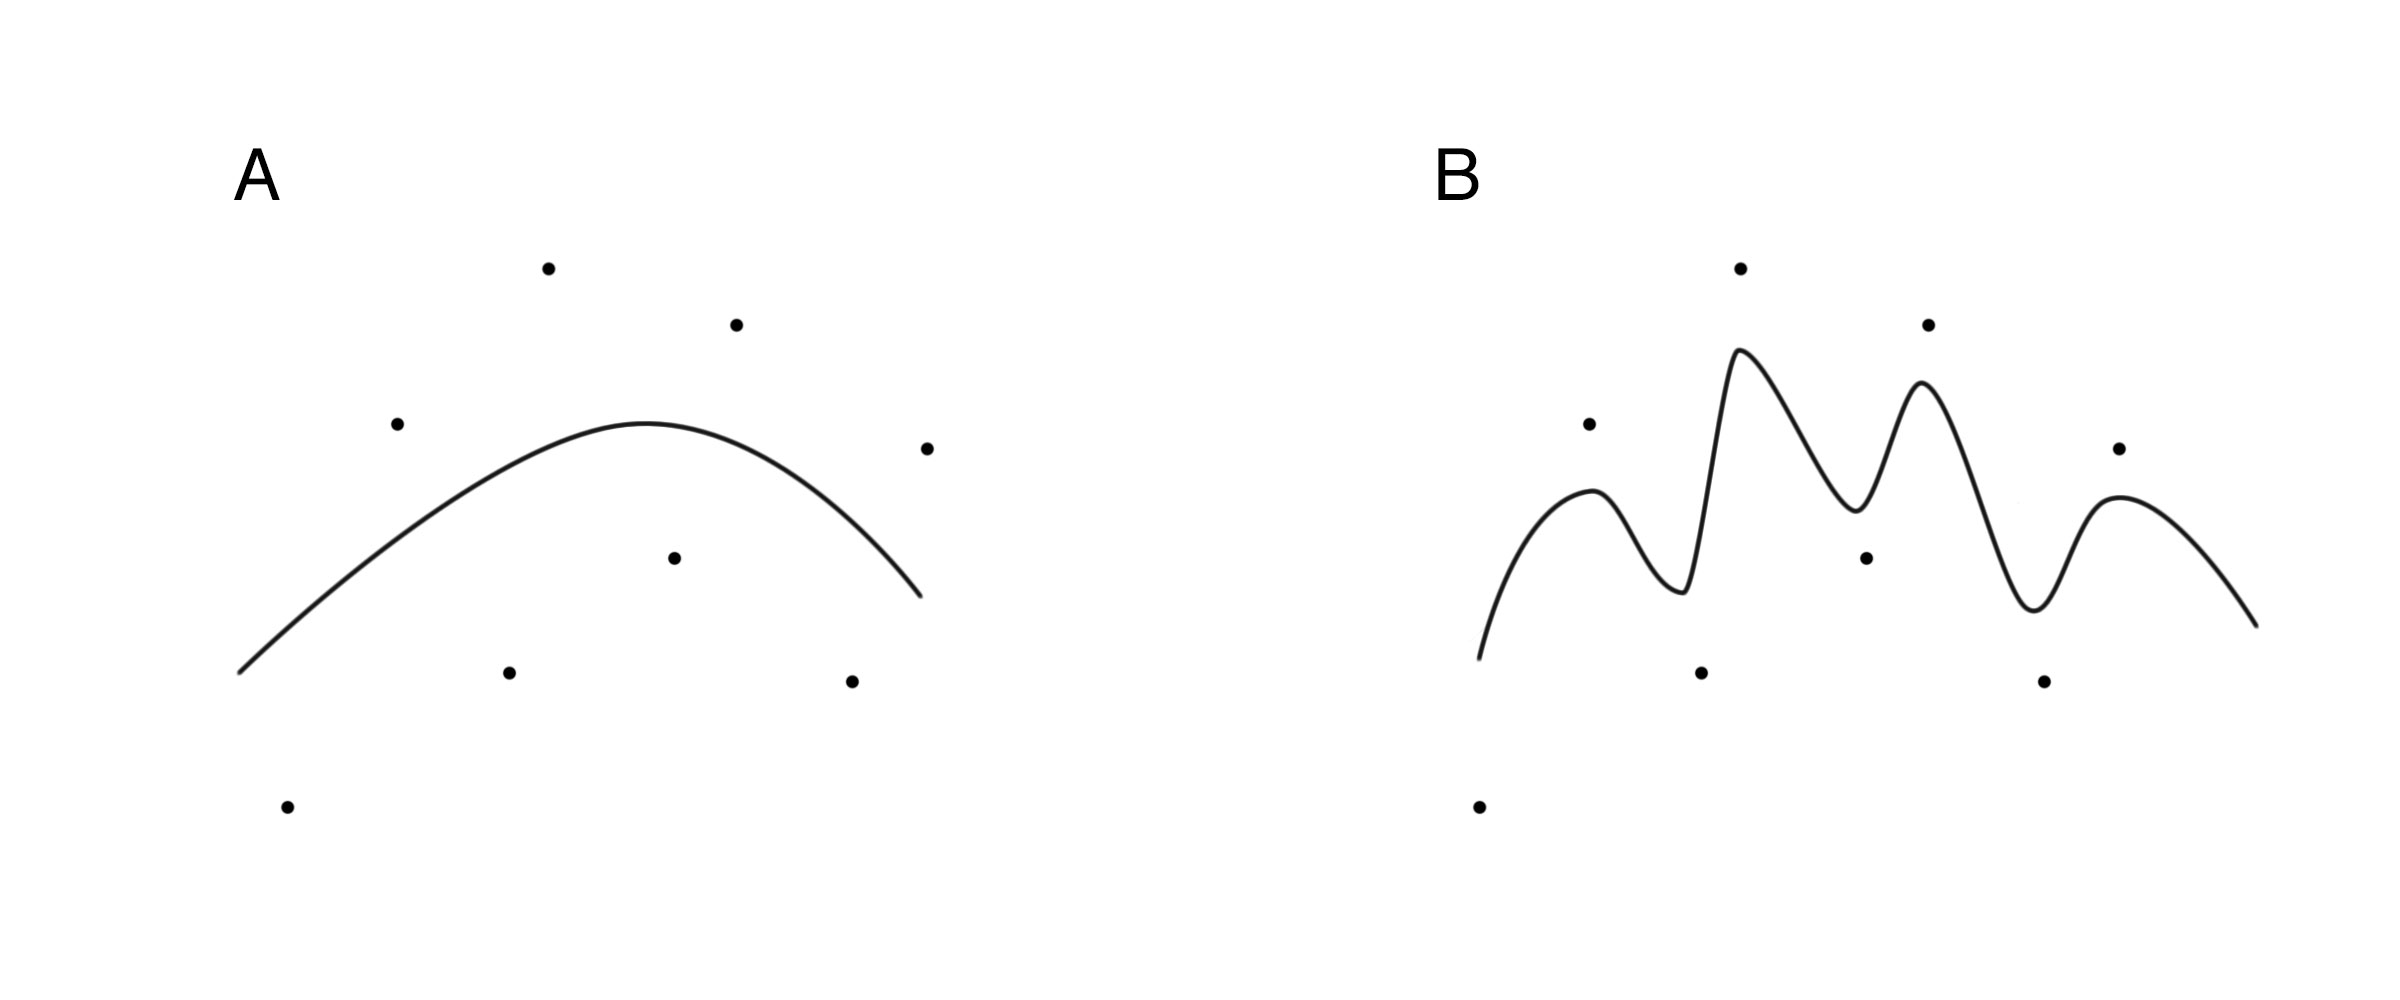
\includegraphics[width=0.99\linewidth,natwidth=898,natheight=587]{billeder/WP_000057.jpg}
\caption{A) Shows the generalized function. B) The approaching of output values}
\label{fig:WP}
\end{figure}

Problems can arise together with the inclusion of tendency --- when have we moved enough in one direction? We need to rely on the other input parameters to help pull us either up or down so that we can identify the next trend if it shifts during the 24-step-ahead prediction. The dataset used for training must be big enough to reflect coming trends or else problems can occur when meeting new trends in the unseen data for prediction, e.g. if most trends in general are rising in the training set and then trying to predict 24 hours that would result in a disproportion between the two sets. The possibility of over-shooting the first targets would be high since it has never seen such trends before. It will need to be tested thoroughly during our experiments. 

One thing to keep in mind here is that the trend and slope are only a minority of the input parameters. Without these the Artificial Neural Network would have made one generalization and the assumptions is that it will help the function to approach the target better when a lot of output possibilities exist. The result will be a new function where the immediate past is considered at every hour and the possibility of a improved generalization. We will experiment with different calculations that identifies something about current behavior. The approaches will be used individually as well as together and will be described in the coming sections.

\subsection{Slope Calculation}
\label{sec:curveAnalysis}
The slope calculation is a simple calculation we created to determine the trend direction of the last X prices/wind productions. It calculates the slope in incremental steps through the stack of historical prices. The results of each calculation is added together and the final result tells us if the gradient has been positive (going up) or negative (going down) in general over the historical values. The reason for calculating the slope in small steps is to avoid generalizing to much. This way every step included in the calculation will have even weight. It is calculated by the following:
\begin{center}
$slope = \sum_{i=1}^{n} y_i - y_{i-1}$
\end{center}
\noindent where y is historical price/wind production.

\subsection{Scatter}
\label{sec:scatterStrategy}
The scatter strategy is a way to let ANN predict the movement of the curve for price/wind production. This methods stands in contrast to the others mentioned here because the others have been precalculated and are represented as a single input. This method involves x-numbers of historical inputs of the price/wind production which we then let the ANN find the correlation between. We have included it to find out if it is more efficient than doing precalculations of the inputs. The inspiration for this method comes from Singhal et al. \cite{singhal2011electricity}. We use the same setup as they propose which includes:

\begin{itemize}
	\item 3 x The price - One day ago
	\item 3 x The price - One week ago
	\item 1 x The price - Two weeks ago
	\item 1 x The price - Three weeks ago
	\item 1 x The price - Four weeks ago
\end{itemize}

\subsection{EWMA - Historical Volatility}
\label{sec:ewmaVolatility}
%\todo{Talk about statistical input features like historical volatility (EWMA), skewness and basic calculation of line slope. Skewness is a more sophisticated way of calculating if the distribution is leaning to one sine of the mean - the %simple line slope calculation is meant to calculate if we are on the way up or down}
EWMA should be used for time series that do not have a clear trend direction\cite[Chapter~7.3.2]{econometrics} which is exactly what we have. \todo{see page 588 in econometrics book}. EWMA is a latent trend model where a latent variable is included to describe a discrete choice model. The latent variable is called the smoothing factor and if this factor is close to one then the last trend has a higher weight than the recent observation and when it is close to zero the new has higher priority and thereby letting the EWMA follow trends more rapidly - in our case the observation would be either production or price and the smoothing factor is calculated based on the last calculated trend. Choice of smoothing factor must be tested in experiments but since there is high volatility in both price and wind power production a lower factor could be expected. Every hour must calculate the historical volatility based on a defined number of previous hours. The exact number will also be found in experiments.

\subsection{Skewness}
\label{sec:skewness}
Skewness is a measure to determine if a variables falls to the left, in the middle or the right of the mean \cite[Chapter~1.1.2]{econometrics}. A skewness calculation on the last X hours uses the distribution of the variables to determine if the predicted value will fall to the left or the right of the median. This is then used to determine the tendency of the slope i.e. if the curve is rising or falling. Skewness is a more sophisticated version of the slope calculation because skewness denotes the probability of what side we are moving to compared to the slope calculation which just calculates a sum of all the gradients.

%TEGNING MULTIPE STEP

%TALK ABOUT MULTIPLE-STEP-AHEAD FORECASTING --> see karlbranting